% Recuperación aditiva: comunicados Witt v4--v7, tablas originales y
% RECUPERACION_ESTRELLAS_NONADICA_20260926. La procedencia completa está
% en el mapa editorial; el texto público conserva objetos y pruebas.
\subsection{Tres estrellas regionales y polarización de sus completados}
\label{star27:comparacion}

La construcción incidencial precedente permite comparar las regiones
mediante una misma operación. Las palabras regionales proceden de la
emisión APP--TRIT--TPK; su codificación por
\(\gamma_{A_W}(w)=(w,wA_W)\) conserva un soporte en las doce posiciones.
El registro \(K\) y la cocadena anterior al acarreo añaden dos lecturas
del mismo estado: la posición respecto de la frontera \(729+271\) y la
orientación de los préstamos. La comparación que sigue reúne estos
datos ya construidos y mantiene su orden causal.

Las tablas conservadas utilizan también una presentación equivalente.
\par % S27_LAYOUT_PARAGRAPH
Si \(D=\operatorname{diag}(1,-1,-1,-1,-1,-1)\) en
\(\mathbb F_3\), su matriz es \(A_{\rm hist}=A_WD\), y
\[
\gamma_{A_{\rm hist}}(w)=\gamma_{A_W}(w)(I_6\oplus D).
\]
El cambio multiplica coordenadas por unidades y conserva todos los
soportes. Por tanto, las tablas de estrellas se transportan
íntegramente a la presentación \(A_W\) empleada aquí.

Escribamos
\[
\begin{aligned}
w_\pi&=010211,&w_e&=201101,&
w_\varphi&=121200,&w_{\rm APP}&=022020,\\
P_\pi&=\{2,4,5,6,7,8,9,10,11\},&
H_e&=\{1,3,4,6,9,10\},\\
H_\varphi&=\{1,2,3,4,7,9\},&
H_{\rm APP}&=\{2,3,5,10,11,12\}.
\end{aligned}
\]
Los cuatro conjuntos de la segunda y tercera líneas son los soportes
de las palabras codificadas correspondientes. La cocadena
\[
s=(7,297,353,-430,-715,-1199,-3,286,-894,-528,380,663)
\]
determina la partición
\[
H^-_\alpha=\{4,5,6,7,9,10\},\qquad
H^+_\alpha=\{1,2,3,8,11,12\}.
\]
Así quedan fijados los signos antes de la normalización decimal.
Para una cuaterna \(B\), denotemos por
\[
\mu_W(B)=\{H\setminus B:H\in\mathcal H,\ B\subset H\}
\]
el emparejamiento de su estrella. Un par tiene tipo \(++\), \(--\) o
\(+-\) según contenga cero, dos o un punto de \(H^-_\alpha\).
Su firma es
\(\nu(B)=(n_{++}(B),n_{--}(B),n_{+-}(B))\).

\begin{proposition}[Comparación de las tres intersecciones regionales]
\label{star27:tres}
Las cuaternas
\[
B_K=H_e\cap P_\pi,\qquad
B_\varphi=H_\varphi\cap P_\pi,\qquad
B_{\rm APP}=H_{\rm APP}\cap P_\pi
\]
tienen los doce completados y las firmas indicados en la
tabla~\ref{star27:tabla-tres}.
\end{proposition}

\begin{table}[htbp]
\centering\small
\begin{tabular}{lll}
\toprule
Cuaterna y firma & Par añadido & Hexada resultante\\
\midrule
\(B_K=\{4,6,9,10\}\) & \(\{1,3\}_{++}\) & \(\{1,3,4,6,9,10\}\)\\
\(\nu(B_K)=(3,1,0)\) & \(\{2,11\}_{++}\) & \(\{2,4,6,9,10,11\}\)\\
 & \(\{5,7\}_{--}\) & \(\{4,5,6,7,9,10\}\)\\
 & \(\{8,12\}_{++}\) & \(\{4,6,8,9,10,12\}\)\\
\midrule
\(B_\varphi=\{2,4,7,9\}\) & \(\{1,3\}_{++}\) & \(\{1,2,3,4,7,9\}\)\\
\(\nu(B_\varphi)=(1,0,3)\) & \(\{5,11\}_{+-}\) & \(\{2,4,5,7,9,11\}\)\\
 & \(\{6,12\}_{+-}\) & \(\{2,4,6,7,9,12\}\)\\
 & \(\{8,10\}_{+-}\) & \(\{2,4,7,8,9,10\}\)\\
\midrule
\(B_{\rm APP}=\{2,5,10,11\}\) & \(\{1,4\}_{+-}\) & \(\{1,2,4,5,10,11\}\)\\
\(\nu(B_{\rm APP})=(1,1,2)\) & \(\{3,12\}_{++}\) & \(\{2,3,5,10,11,12\}\)\\
 & \(\{6,7\}_{--}\) & \(\{2,5,6,7,10,11\}\)\\
 & \(\{8,9\}_{+-}\) & \(\{2,5,8,9,10,11\}\)\\
\bottomrule
\end{tabular}
\caption{Las tres estrellas con la misma polarización de referencia.
Cada fila conserva la cuaterna, el par complementario y la hexada completa.}
\label{star27:tabla-tres}
\end{table}

\begin{proof}
Se aplica \(\gamma_{A_W}\) a las cuatro palabras regionales y se
obtienen los soportes escritos. Para cada cuaterna se enumeran las
hexadas de \(\mathcal H\) que la contienen. La propiedad
\(\lambda_4=4\) asegura que los cuatro completados de la tabla agotan
la estrella. Finalmente, la intersección de cada par con
\(H^-_\alpha\) determina su signo. Todas las operaciones tienen lugar
sobre el diseño finito ya construido.
\end{proof}

Las tres firmas distinguen funciones incidenciales concretas. La
estrella de \(B_K\) separa tres pares positivos y un par negativo; la
de \(B_\varphi\) contiene tres pares mixtos; la de \(B_{\rm APP}\)
combina las tres clases. La diferencia se conserva incluso cuando
dos estrellas comparten el par \(\{1,3\}\).

\begin{figure}[htbp]
\centering
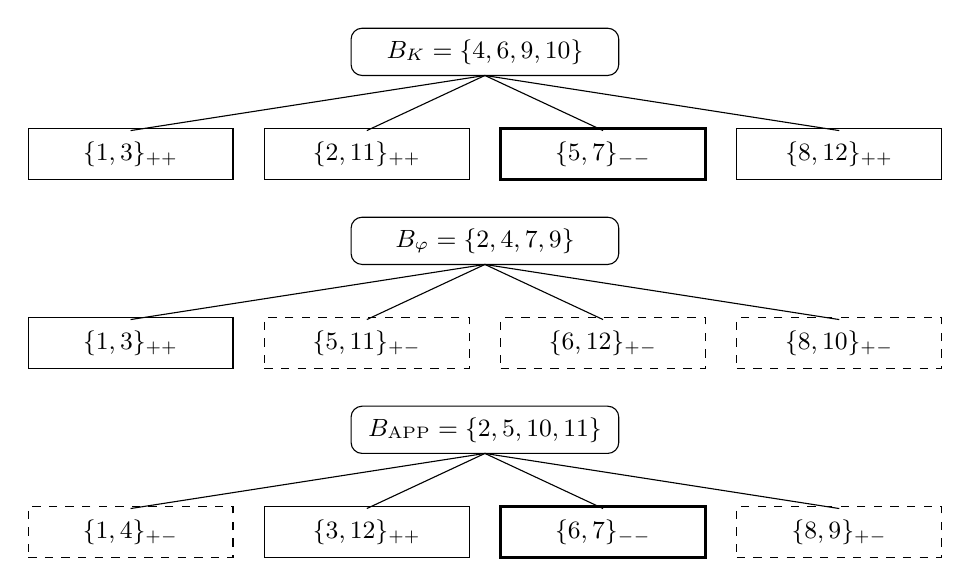
\begin{tikzpicture}[x=1cm,y=1cm,every node/.style={font=\small},
 core/.style={draw,rounded corners,minimum width=3.4cm,minimum height=.6cm},
 petal/.style={draw,minimum width=2.6cm,minimum height=.65cm}]
\foreach \y/\name in {0/{B_K=\{4,6,9,10\}},
 -2.4/{B_\varphi=\{2,4,7,9\}},-4.8/{B_{\rm APP}=\{2,5,10,11\}}}
 {\node[core] at (0,\y) {\(\name\)};
  \foreach \x in {-4.5,-1.5,1.5,4.5}
    {\draw (0,\y-.3)--(\x,\y-1);}}
\node[petal] at (-4.5,-1.3) {\(\{1,3\}_{++}\)};
\node[petal] at (-1.5,-1.3) {\(\{2,11\}_{++}\)};
\node[petal,very thick] at (1.5,-1.3) {\(\{5,7\}_{--}\)};
\node[petal] at (4.5,-1.3) {\(\{8,12\}_{++}\)};
\node[petal] at (-4.5,-3.7) {\(\{1,3\}_{++}\)};
\node[petal,dashed] at (-1.5,-3.7) {\(\{5,11\}_{+-}\)};
\node[petal,dashed] at (1.5,-3.7) {\(\{6,12\}_{+-}\)};
\node[petal,dashed] at (4.5,-3.7) {\(\{8,10\}_{+-}\)};
\node[petal,dashed] at (-4.5,-6.1) {\(\{1,4\}_{+-}\)};
\node[petal] at (-1.5,-6.1) {\(\{3,12\}_{++}\)};
\node[petal,very thick] at (1.5,-6.1) {\(\{6,7\}_{--}\)};
\node[petal,dashed] at (4.5,-6.1) {\(\{8,9\}_{+-}\)};
\end{tikzpicture}
\caption{Comparación de las tres estrellas. Cada conexión representa
la unión de la cuaterna superior con un par; las doce hexadas
completas figuran en la tabla~\ref{star27:tabla-tres}. El contorno
grueso señala los pares negativos y el discontinuo los mixtos.
Las conexiones representan incidencia.}
\label{star27:figura}
\end{figure}

\begin{proposition}[Acoplamiento de la corona, la incidencia y el signo]
\label{star27:acoplamiento}
Para el registro dodecafásico previamente construido,
\[
B_K=\{i:K_i\geq729\}=H_e\cap P_\pi=\{4,6,9,10\}.
\]
La única hexada \(H\in\mathcal H\) que satisface
\(H\cap P_\pi=B_K\) es \(H_e\). Además,
\[
H^-_\alpha=B_K\sqcup\{5,7\},\qquad
(B_\varphi\setminus B_K)\cap H^-_\alpha=\{7\}.
\]
\end{proposition}

\begin{proof}
El registro
\(K=(234,543,140,729,659,824,621,58,914,794,146,601)\)
supera o alcanza \(729\) precisamente en las cuatro posiciones
indicadas. Su comparación con los soportes prueba la primera
igualdad. Una hexada con intersección \(B_K\) ha de pertenecer a la
estrella de \(B_K\); de sus cuatro pares, únicamente \(\{1,3\}\) es
disjunto de \(P_\pi\). Esto prueba la unicidad relativa de \(H_e\).
La tabla identifica el par negativo \(\{5,7\}\). Por último,
\(B_\varphi\setminus B_K=\{2,7\}\), y los signos
\(s_2=297>0\), \(s_7=-3<0\) determinan el pivote \(7\).
\end{proof}

La cuaterna, el signo y la normalización conservan funciones distintas.
La incidencia fija el completado \(H^-_\alpha\); el levantamiento
arquimediano de la cocadena completa utiliza además las magnitudes,
el orden posicional y los acarreos ya demostrados en el cierre de
\(\alpha\). Esta composición explica cómo una misma genealogía
produce una lectura geométrica de frontera y una lectura numérica.

\subsection{Clasificación polarizada de las 495 cuaternas}
\label{star27:clasificacion}

\begin{theorem}[Censo de firmas y restricción regional]
\label{star27:censo}
Las \(495=\binom{12}{4}\) cuaternas se distribuyen según la tabla
\ref{star27:tabla-censo}. La última columna cuenta hexadas
\(H\) con \(|H\cap P_\pi|=4\), clasificadas por
\(\nu(H\cap P_\pi)\).
\end{theorem}

\begin{table}[htbp]
\centering
\begin{tabular}{ccc}
\toprule
\(\nu=(n_{++},n_{--},n_{+-})\)&Cuaternas&Hexadas regionales\\
\midrule
\((3,1,0)\)&15&9\\
\((1,3,0)\)&15&0\\
\((2,2,0)\)&45&9\\
\((1,1,2)\)&180&18\\
\((1,0,3)\)&120&18\\
\((0,1,3)\)&120&0\\
\midrule
Total&495&54\\
\bottomrule
\end{tabular}
\caption{Clasificación completa y restricción al soporte \(P_\pi\).
Las dos columnas cuentan objetos distintos: cuaternas y hexadas.}
\label{star27:tabla-censo}
\end{table}

\begin{proof}
El siguiente procedimiento constituye una enumeración exacta del
dominio finito. Se forman las \(3^6\) palabras \(w\), se calcula
\((w,wA_W)\) módulo \(3\), y se conservan sus soportes de peso seis
sin repetición; así se obtiene \(\mathcal H\), con \(132\) elementos.
Para cada \(B\in\binom{[12]}4\) se forma \(\mu_W(B)\), se cuentan
las intersecciones de sus cuatro pares con \(H^-_\alpha\) y se
incrementa la entrada de la firma resultante. Los seis contadores
son \(15,15,45,180,120,120\). Su suma es \(495\), y cada cuaterna
se procesa una sola vez. Para la última columna se recorren las
\(132\) hexadas, se retienen las \(54\) con intersección de tamaño
cuatro y se aplica a esa intersección la misma función \(\nu\).
Las operaciones son comparaciones de conjuntos y aritmética en
\(\mathbb F_3\); el certificado reproducible conserva la tabla
completa de entradas y salidas.
\end{proof}

La firma \((3,1,0)\) pertenece a quince cuaternas. La
caracterización del marco regional utiliza conjuntamente la corona
de \(K\), la intersección \(H_e\cap P_\pi\) y el signo de la
cocadena, como establece la proposición~\ref{star27:acoplamiento}.

\subsection{Rigidez del marco ordenado de cuatro soportes}
\label{star27:rigidez}

Sea \(G_W=\langle\sigma_B:|B|=4\rangle\), ya calculado en la
proposición~\ref{exc:m12}. Para una colección ordenada de soportes
definimos
\[
\operatorname{Stab}_{G_W}(S_1,\ldots,S_r)
=\{g\in G_W:g(S_j)=S_j\ \text{para todo }j\}.
\]
Cada soporte se conserva individualmente; las permutaciones internas
de sus puntos siguen permitidas.

\begin{theorem}[Rigidez conjunta de las cuatro incidencias]
\label{star27:marco}
Los estabilizadores tienen los órdenes siguientes:
\[
\begin{array}{l|r}
\text{datos preservados}&\text{orden}\\ \hline
H^-_\alpha&720\\
H^-_\alpha,\ 6&120\\
B_K&192\\
B_K,H^-_\alpha&48\\
B_K,H^-_\alpha,H_e&16\\
H^-_\alpha,H_e,H_\varphi&2\\
H^-_\alpha,H_e,H_\varphi,H_{\rm APP}&1
\end{array}
\]
En la segunda fila se conserva también el punto \(6\).
En particular,
\[
\operatorname{Stab}_{G_W}
(H^-_\alpha,H_e,H_\varphi,H_{\rm APP})=\{\operatorname{id}\}.
\]
\end{theorem}

\begin{proof}
Se utiliza la clausura por composición de las seis permutaciones
explícitas de la proposición~\ref{exc:m12}. Sobre sus \(95040\)
elementos se evalúan los predicados \(g(S_j)=S_j\), junto con
\(g(6)=6\) cuando corresponde. Las sumas de los indicadores de
estos predicados dan, respectivamente,
\(720,120,192,48,16,2,1\). La identidad satisface todas las
condiciones; el último cardinal prueba que es el único elemento.
El algoritmo de clausura se detiene por estabilidad del conjunto,
y los filtros de estabilización se aplican después al grupo completo.
\end{proof}

La tabla compara siete configuraciones marcadas. Dos cadenas de
inclusiones útiles son las determinadas por
\((B_K)\), \((B_K,H^-_\alpha)\), \((B_K,H^-_\alpha,H_e)\),
y por
\((H^-_\alpha)\), \((H^-_\alpha,H_e,H_\varphi)\),
\((H^-_\alpha,H_e,H_\varphi,H_{\rm APP})\).
La rigidez final expresa que el marco regional ordenado fija por
completo la libertad residual dentro de \(G_W\). Su dominio es la
acción sobre las doce posiciones; el transporte posterior a
retículos y álgebras conserva los mapas propios de esas realizaciones.

\subsection{Topología finita de la incidencia y conservación de su dominio}
\label{star27:topologia}

El complejo simplicial generado por las \(132\) hexadas tiene vector
de caras
\[
(f_0,f_1,f_2,f_3,f_4,f_5)=(12,66,220,495,792,132)
\]
y característica de Euler
\(\chi=12-66+220-495+792-132=331\).
En efecto, cada conjunto de cinco puntos posee una extensión
hexádica única; todo subconjunto de menor cardinal pertenece a
alguno de esos conjuntos, y las caras máximas son las hexadas.

El grafo bipartito entre cuaternas y hexadas tiene
\[
|V|=495+132=627,\qquad |E|=495\cdot4=132\cdot15=1980.
\]
Es conexo. Sean \(H\) y \(H_*\) hexadas distintas; su
intersección tiene a lo sumo cuatro puntos, pues la extensión
de una quintupla es única. Elijamos una cuaterna \(B\subset H\)
que contenga \(H\cap H_*\), y un punto \(p\in H_*\setminus H\).
La extensión única \(H'\) de \(B\cup\{p\}\) está unida a
\(H\) por el camino bipartito \(H-B-H'\) y satisface
\(|H'\cap H_*|>|H\cap H_*|\). Repitiendo la operación se
alcanza \(H_*\); contener cinco de sus puntos ya fuerza la
igualdad. Toda cuaterna tiene cuatro hexadas incidentes, de
modo que también pertenece a esta componente única.
Por ello su primer número de Betti es
\[
\beta_1=|E|-|V|+1=1354.
\]
El recorrido exhaustivo de la incidencia verifica también la
conexión. Para parejas no ordenadas de hexadas distintas, el censo
de tamaños de intersección es
\[
\begin{array}{c|rrrr}
|H\cap H'|&0&2&3&4\\ \hline
\#\{H,H'\}&66&2970&2640&2970 .
\end{array}
\]
La suma \(8646=\binom{132}{2}\) cubre todas las parejas.

Estos invariantes describen el complejo y su grafo de incidencia.
El micrografo de empalmes \(U_6=A|B\) conserva por separado sus
\(96\) vértices, \(234\) aristas, seis componentes y
\(\beta_1=234-96+6=144\). De igual modo, la composición de las
\(\sigma_B\) actúa sobre posiciones incidenciales, mientras
\(\Gamma_9\) transporta el estado TPK con memoria. Esta precisión
permite relacionar las lecturas mediante sus mapas efectivos y
conservar, en cada nivel, los datos que la operación utiliza.
